\localauthor{Stefanie Gürster}
\subsection{Benutzeroberfläche}

\subsection{Benutzerfluss}
Im Folgenden werden functioning Aussagen über die Benutzeroberfläche mithilfe eines Benutzerflussdiagramms getroffen.

\begin{figure}[H]
    \centering
    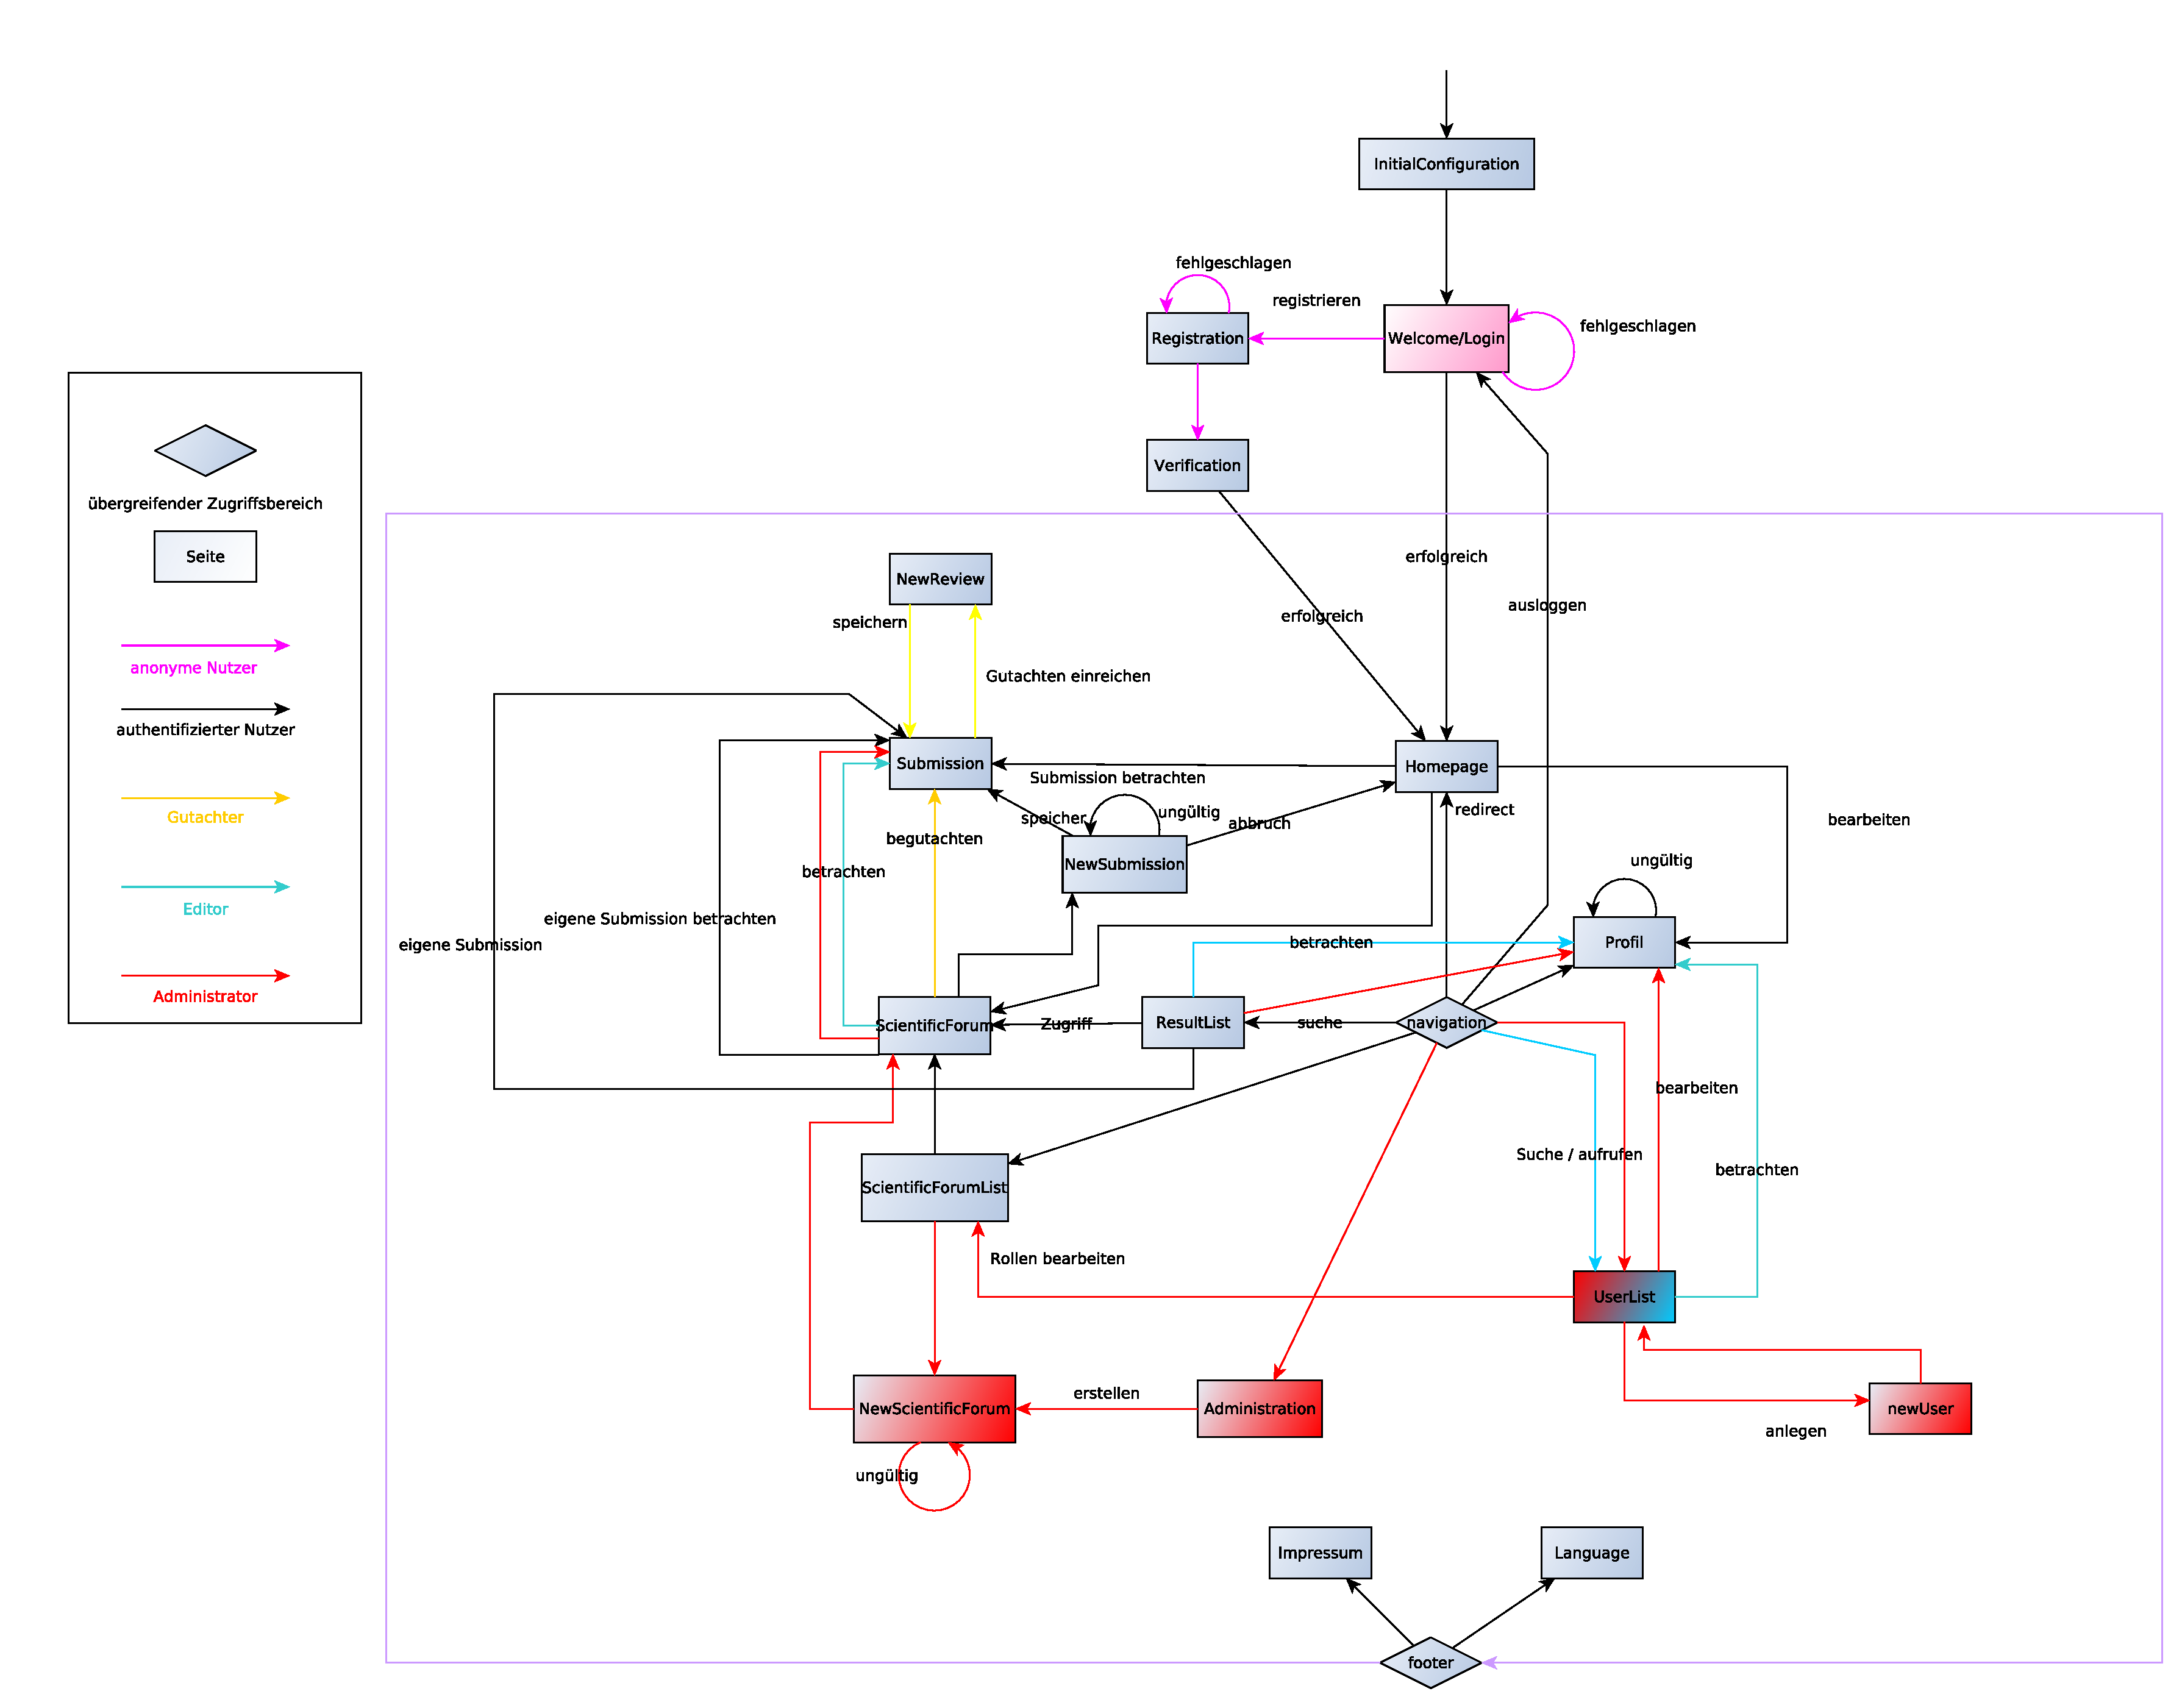
\includegraphics[width=\linewidth]{graphics/benutzerFlussyEd}
    \caption{Benutzerfluss}
\end{figure}

Die sich im Diagramm befindlichen Rauten stellen Header (Navigationsleiste) und Footer dar.
Hierbei wird jedoch wie folgt unterschieden: Der Header ist nur für authentifizierte Nutzer:innen zugänglich,
d.h. dieser erscheint erst nach einem erfolgreichen Login sichtbar und verschwindet nach einem Logout wieder.
Der Footer hingegen ist von jeder Seite der Applikation zugänglich und somit sichtbar.

Im Diagramm werden Administratoren, Editoren, Gutachter und normale Nutzende unter dem allgemeinen Begriff
authentifizierte Nutzer:innen betrachtet.
Sind die Verbindungspfeile nicht schwarz, sondern andersfarbig dargestellt besitzen auch nur die
dargestellten Benutzergruppen ein Zugriffsrecht oder das Recht auf eine Aktion.

Des Weiteren ist der Randfall zu betrachten, bei welchem ein externer Gutachter, welcher noch nicht registriert ist,
eine Einladung eines Editors angenommen hat.
Diesem wird die Rolle eines Gutachters zugewiesen, jedoch besitzt er erst Zugriffsrechte, nachdem er sich
authentifiziert hat.